\subsection{Longer windows, nested liquid universes and forward diagnostics}\label{sec:extended}
The full-panel result motivates a sensitivity analysis that separates sample length from changing stock composition. Before computing the extended outcomes, we fixed the last recorded origin in every represented calendar year, giving 19 annual origins. The complete retrospective sensitivity grid and its unavailable cases are reported. At each origin, we use the longest calendar-available lookback from 504 and 1008 sessions to screen the original eligible list. Eligibility requires complete past returns, supplied prices and volumes, positive volume on at least 90\% of sessions, at most 15\% zero returns, and positive variance. Within this eligible set we rank stocks by median supplied closing price times volume, breaking ties by ISIN. This is an available-data liquidity proxy, not a certified corporate-action-adjusted traded-value measure.

We take nested groups of 10, 20 and 40 stocks. Their membership is kept fixed when comparing 252, 504 and 1008 sessions at the same origin. Changing group size changes the population tree target; a hub of a small liquid subnetwork need not be a hub of the full market. Demeaning is recomputed within each selected group, while factor residualization retains the same WIG series. All dated observations used for selection precede or coincide with the origin; future observations never enter selection. Vendor histories can incorporate later revisions, so this rule does not establish a fully point-in-time data source.

Of 513 planned origin--lookback--group--representation combinations, 81 cannot be evaluated because of insufficient calendar history or too few eligible stocks. We retain the full exclusion list. The remaining 432 primary analyses use block length ten and 999 common-row resamples per origin and lookback, across all three representations. A further 34 raw-network analyses examine block lengths five and twenty at $p=20,n=1008$, for all 17 available origins. These are nominal, per-configuration bootstrap projections. We do not claim simultaneous coverage over the grid or valid 95\% coverage for dependent returns.

\begin{table}[htbp]
\caption{Raw-network comparison on identical stocks and matched origins. The 1008-session availability criterion leaves 17 origins for groups of 10 and 20, and ten for groups of 40. Widths and forced-edge counts are within-group origin averages. Full ranks is the fraction of vertex ranges remaining $[1,p]$.}\label{tab:extended}
\centering\small
\begin{tabular}{rrrrrr}
\toprule
$p$ & Origins & $n$ & Degree width & Forced edges & Full ranks \\
\midrule
10 & 17 & 252 & 6.71 & 0.47 & 1.00 \\
10 & 17 & 504 & 6.18 & 0.59 & 1.00 \\
10 & 17 & 1008 & 5.78 & 1.00 & 1.00 \\
20 & 17 & 252 & 15.04 & 0.47 & 1.00 \\
20 & 17 & 504 & 14.14 & 0.65 & 1.00 \\
20 & 17 & 1008 & 12.92 & 1.35 & 1.00 \\
40 & 10 & 252 & 32.82 & 0.00 & 1.00 \\
40 & 10 & 504 & 31.03 & 0.20 & 1.00 \\
40 & 10 & 1008 & 29.45 & 0.80 & 1.00 \\
\bottomrule
\end{tabular}
\end{table}
The matched-origin mean degree width decreases by 13.9\%, 14.1\% and 10.3\% when moving from 252 to 1008 observations for groups of 10, 20 and 40 respectively. More edges are forced under the nominal order region, but none of the 432 primary or 34 block-sensitivity configurations yields a non-full vertex rank interval or a certified unique hub. The negative ranking result therefore survives a fourfold lookback extension, liquidity-based dimension reduction, and the stated block checks. This describes resolution for the stated procedures and targets.

\begin{table}[htbp]
\caption{Block-length sensitivity for the same 17 raw-network origins, $p=20,n=1008$. Resampling seeds differ between block lengths.}\label{tab:blocks}
\centering\small
\begin{tabular}{rrrrr}
\toprule
Block length & Origins & Degree width & Forced edges & Full ranks \\
\midrule
5 & 17 & 12.94 & 1.24 & 1.00 \\
10 & 17 & 12.92 & 1.35 & 1.00 \\
20 & 17 & 12.93 & 1.29 & 1.00 \\
\bottomrule
\end{tabular}
\end{table}
For a forward diagnostic, we hold the training stock group fixed and estimate a new tree using the next 252 sessions. The diagnostic is available only when every selected stock and the factor have complete future returns. We neither impute unavailable histories nor drop a future-missing stock from the selected group. There are 93 complete primary configurations per representation, out of 144; the remaining 51 have incomplete future histories or insufficient follow-up. Overlapping lookbacks and nested groups mean these are not 93 independent samples. Forward summaries are conditional on future-history availability and may be affected by attrition; no reweighting corrects that selection. We compute the fraction of transitive training order statements whose direction agrees with the future correlation estimates, and whether the training anchor remains tied for largest future degree. These are descriptive temporal-stability measures, not population coverage tests or portfolio-performance results.

\begin{table}[htbp]
\caption{Forward diagnostics over the next 252 sessions. Order agreement averages the within-configuration fractions, giving each configuration equal weight. Anchor still top includes ties and does not establish a unique hub.}\label{tab:forward}
\centering\small
\begin{tabular}{lrrr}
\toprule
Representation & Configurations & Order agreement & Anchor still top \\
\midrule
Raw & 93 & 95.7\% & 35/93 \\
Demeaned & 93 & 95.2\% & 19/93 \\
WIG residual & 93 & 93.9\% & 19/93 \\
\bottomrule
\end{tabular}
\end{table}
Estimated edge-order directions persist much more frequently than the identity of the estimated highest-degree vertex. This comparison involves different functionals: preservation of many inequalities is not equivalent to preservation of a hub, and a high fraction of correct directions need not mean that every direction is preserved jointly. Because the population can change over time, the forward sample is not a known-truth coverage benchmark. The calibration failures in Section~\ref{sec:simulation} remain unresolved.

As an illustration, the earliest complete raw-network configuration with anchor bootstrap frequency at least 0.9 and loss of top position in the future sample is the 2008 annual origin, $p=10,n=504$. The anchor is PKOBP; it is tied for highest degree in 91.2\% of bootstrap trees, while its nominal degree range is [1, 9] and rank range is [1, 10]. Its future estimated rank range is [3, 10], despite 100.0\% directional agreement for the certified training orders. The illustration is selected retrospectively by the stated rule; all configurations are reported, and it is not additional confirmatory evidence.

\begin{figure}[htbp]\centering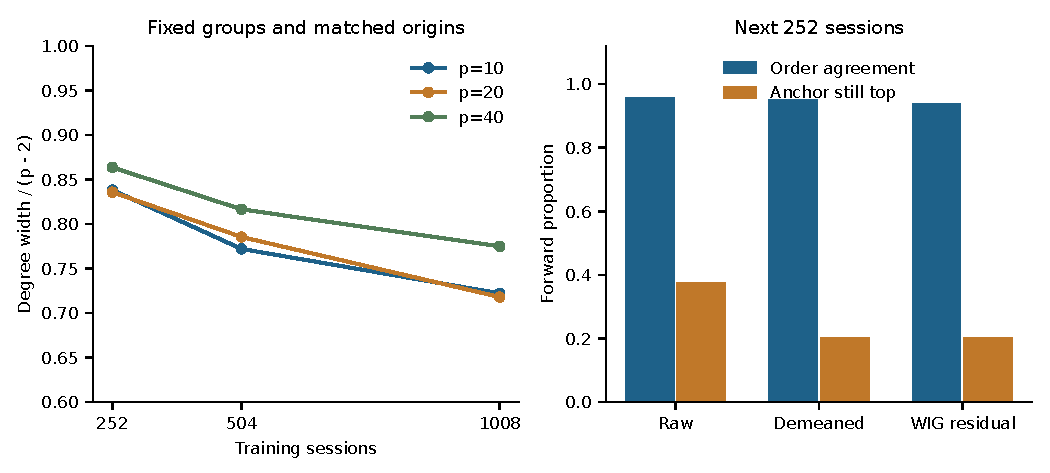
\includegraphics[width=\textwidth]{Fig_empirical.pdf}\caption{Extended empirical diagnostics. Left: mean raw-network degree width divided by $p-2$, on the matched origins and fixed stock groups in Table~\ref{tab:extended}. Right: forward edge-order agreement and retention of the training anchor among the highest-degree vertices, from Table~\ref{tab:forward}. Both panels are descriptive; neither supplies a validated confidence level for GPW returns.}\label{fig:empirical}\end{figure}
Independent verification reconstructs the selection rule for all 50 origin--group universes, checks five source-input hashes and all 9,710 additional vertex records, recomputes the 303 available forward analyses including block sensitivities, and validates all 24,419 improving rational LP certificates. Every check passes. Longer financial windows increase sample size while raising the possibility of regime changes, so their improved degree resolution must be interpreted alongside that stationarity limitation.
